\documentclass[conference,compsoc,a4paper]{IEEEtran}
\ifCLASSOPTIONcompsoc
  \usepackage[nocompress]{cite}
\else
  \usepackage{cite}
\fi

\usepackage{array}
\usepackage[utf8]{inputenc}   % <<<<< Linux
\usepackage[nomain,acronym,xindy,toc]{glossaries} 
\usepackage{dirtytalk}
\usepackage{graphicx}
\usepackage{tabularx} 
\usepackage{hyperref}
%Includes "References" in the table of contents
%\usepackage[nottoc]{tocbibind}


\hyphenation{op-tical net-works semi-conduc-tor}
\loadglsentries[main]{xacronyms}
\begin{document}

\newcolumntype{Y}{>{\centering\arraybackslash}X}
\newcolumntype{M}[1]{>{\centering\arraybackslash}m{\linewidth/#1}}

\title{Hyper-linked Communications: WebRTC enabled asynchronous collaboration}

\author{\IEEEauthorblockN{Michael Shell}
\IEEEauthorblockA{School of Electrical and\\Computer Engineering\\
Georgia Institute of Technology\\
Atlanta, Georgia 30332--0250\\
Email: http://www.michaelshell.org/contact.html}
\and
\IEEEauthorblockN{Homer Simpson}
\IEEEauthorblockA{Twentieth Century Fox\\
Springfield, USA\\
Email: homer@thesimpsons.com}
\and
\IEEEauthorblockN{James Kirk\\ and Montgomery Scott}
\IEEEauthorblockA{Starfleet Academy\\
San Francisco, California 96678-2391\\
Telephone: (800) 555--1212\\
Fax: (888) 555--1212}}

\maketitle

\begin{abstract}

The Hyper-linked communications concept applies much of the hypermedia concepts, widely used on Web content. This paradigm allows to synchronize, structure and navigate communication content integrated into voice and video calls.

Voice and image together can express emotions like no other medium can. With hypermedia concepts, we can add more value to conference calls.

\emph{WebRTC} technology allows real-time communications between web browsers without the need to install additional software. The nature of web browser applications already follows the hypermedia concept, which makes \emph{WebRTC} the ideal technology to apply the hyper-linked communications concepts.
The web browser platform provides an abstraction layer that makes it possible to create applications that run independently from the operating system.
The native support for \emph{WebRTC} in operating systems extends its usage to outside the web browser, allowing for the exploration of functionalities for which web browsers provide poor support, such as video recording and massive information storage.

Our goal was the development of an application targeted to the web platform, resorting to \emph{WebRTC}, that leveraged the hyper-linked communications by providing a conference environment enriched with multiple media types, collaborative text editors, time annotations, instant messaging and a mechanism to superimpose hyper-content to video.

In this document, we present the current State Of The Art in hyper-linked communications and related technologies, propose and implement an architecture for an hyper-linked communication application based on \emph{WebRTC}. This work was evaluated by users, who reported that they liked to use it and thought it to be extremely innovative. 

\end{abstract}

\IEEEpeerreviewmaketitle

\section{Introduction}
\label{chapter:introduction}

\subsection{Background}
\label{section:background}

	As communications technologies appeared, we adapted the way we communicate. The purpose of this project is not the replacement of the current video and audio communications, but to enrich them with hyper-media content and make them a more natural and easy to learn process. 

	With the advent of WebRTC and its successive integration with web browsers, it became possible to develop video conference web applications without plugins, this presents a range of possibilities on what can be implemented using already existing web technologies.
		
    Furthermore, real-time communication applications can make a significant difference on business, education and health sectors by providing tools for developing teaching and learning online, teamworking and socializing web applications.

\subsection{Proposed Solution}
\label{section:proposed}

	Our goal in this project is to develop an application targeted to the web platform, resorting to \gls{WebRTC}, that leverages the hyper-linked communications by providing a video conference environment enriched with interactive and non-interactive discrete media types such as images, subtitles, forms and all types of content that can be added using \gls{HTML}5, \gls{CSS}3 and \emph{JavaScript} including continuous media types such as video, music and animations.

	One of the key features of this project is the ability to navigate in time in order to reproduce the conversation again or introduce hyper-content to it such as time annotations, interactive lists of topics and subtitles. In this context we also provide a simpler method for creating and synchronizing hyper-content using \emph{QR codes}.

	In addition to this conference environment, which provides different functionalities than traditional conference environments such as \emph{Skype} and \emph{Google Hangouts}, we also enable a collaborative text editor and a chat that supports sending time hyper-links and files to conference participants.

	Furthermore, another relevant feature is the possibility to compose multiple video streams into a single one, which enables adding more users to conference rooms without impacting on clients performance. Users can change to individual streams on demand or automatically to the talking users.
        

\subsection{Thesis Contribution}
\label{section:contribution}

Making it clear, this project aims to complement current audio, text and video communications in order to create rich and collaborative interfaces with the ability to add more content on a future time (e.g. creating time annotations for improving content search) in order to increase its value. It is also important to highlight another goal of this project which is the ability to navigate in time by rewinding communications, fast-forward and jump to certain points.

	We have presented an architecture that can meet our goals, implemented the respective prototype and tested it with real users and performance benchmarks.

	According to Martin Geddes, the quality of the interaction worsens as the number of users increase\cite{geddes}. In our testing phases we will quantify and qualify the impact of increasing users on the interface and performance of our prototype. 

	All the problems faced during the development and limitations were reported on the thesis so that a future project better then ours can be easily and better developed.

\subsection{Outline}

This rest of this document is structured as follows:

\begin{itemize}

\item \textbf{Chapter \ref{chapter:relatedwork}} describes the previous work in the field.
\item \textbf{Chapter \ref{chapter:architecture}} describes the system requirements and the architecture for an Web Application that fulfills the goals of this thesis.
\item \textbf{Chapter \ref{chapter:implementation}} describes the implementation of our Web Application and the technologies chosen.
\item \textbf{Chapter \ref{chapter:evaluation}} presents the evaluation tests performed and the corresponding results.
\item \textbf{Chapter \ref{chapter:conclusion}} summarizes the work developed and proposes future work.
\end{itemize}

\section{Related Work}
 This section is structured as follows.
 Section \ref{early} describes the problems that real-time communications face on nowadays internet, namely the \gls{IPv4} address exhaustion and the client server model constraints. 
 Section \ref{rtc} describes the \gls{WebRTC} technology and the protocols needed to implement our project. 
 Section \ref{signaling} addresses the signaling component of chat applications, which is not defined on \gls{WebRTC} specifications. 
 Section \ref{hypermedia} presents the evolution of multimedia content until the hypermedia, its capabilities, synchronization mechanisms and interactivity. 
 Section \ref{collab} explores streaming protocols for non-interactive multimedia and how to introduce the interactive component, another important aspects are the ability to control the time flux of a stream and collaborative application development.
        

\subsection{Early days of the Internet and its remaining flaws}\label{early}

The need to build a global communications network in an age when almost nobody had access to that technology and the unpredictability of the number of future users, lead to some protocols not being suitable for the explosive growth and proliferation of users that followed. \gls{IPv4} limits the number of public addresses in such a way that today they are scarce \cite{ipv4}. 

To this end, one way to overcome the \gls{IPv4} address scarcity problem was the development of a mechanism that groups multiple address into a single one, the machine that is assigned that address is then responsible for redirecting messages to members of its group using their private addresses, each connection in the private network is identified publicly by the same \gls{IP} address with a different port.

This technique is known as \gls{NAT} (figure \ref{fig:nat}).

\begin{figure}
	\centering
	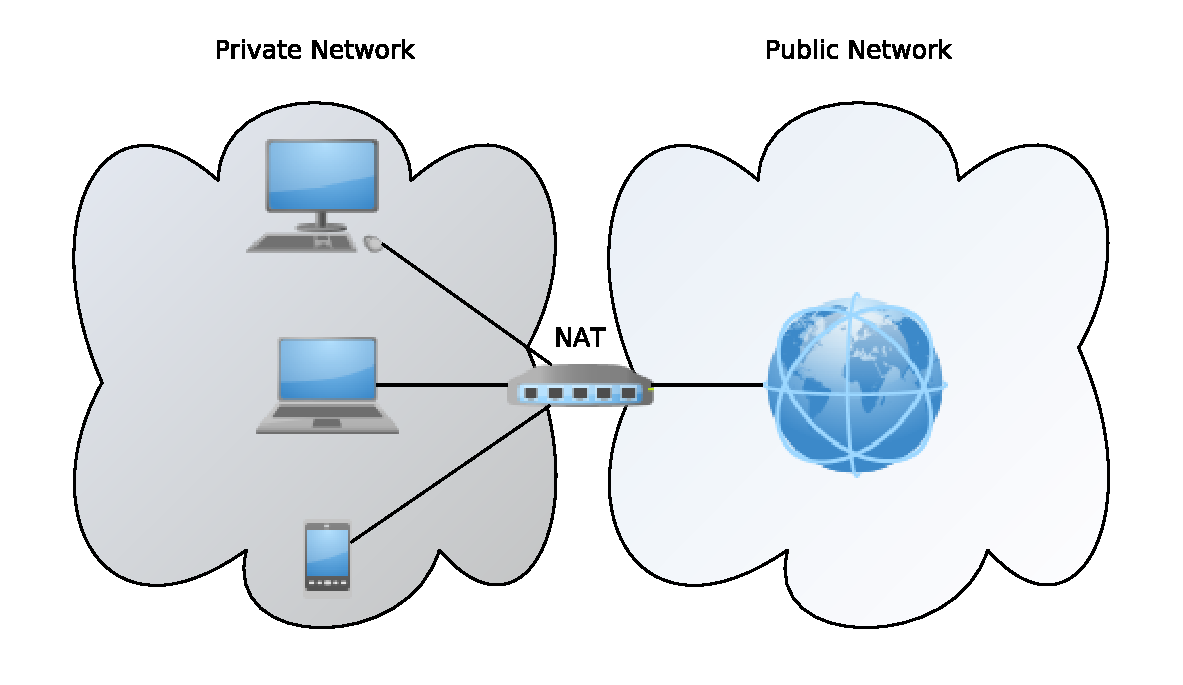
\includegraphics[width=\linewidth]{figures/nat.pdf}
	\caption{Network Address Translation}
	\label{fig:nat}
\end{figure}

Initially \gls{NAT} offered an alternative to address exhaustion and a minimal sensation of security.
However, due to their current wide usage, \gls{NAT}s weaknesses are being exposing at the application layer, namely impacting applications that require direct communications between two private networks.

There are four types of \gls{NAT} implementations\cite{rfc3489}: \emph{Full Cone NAT}, \emph{Restricted Cone NAT}, \emph{Port Restricted Cone NAT}, \emph{Symmetric NAT}.

\emph{Full Cone} \gls{NAT} maps each public \gls{IP} address and port to a private \gls{IP} address and port.
Any external host can communicate with private hosts through their mapped public address and port. This represents the least restrictive type of \gls{NAT} and, as we will see later, the unique type of \gls{NAT} that enables real time communications from point to point.

\emph{Restricted Cone} \gls{NAT} requires that a private client must first send a message to an external host before it can receive messages from the same host. With this type of \gls{NAT}, the private client can be contacted from any port of the same external host.

\emph{Port Restricted Cone} \gls{NAT} works in the same way as Restricted Cone \gls{NAT}, but it only allows communications from the same external host's IP address and port, ignoring all messages from other applications within the same external host.

\emph{Symmetric} NAT maps different ports for each connection. As we will see later, this type of \gls{NAT} represents a problem on real time communications.

\emph{Non-Symmetric} \gls{NAT}s became the common configurations on the Internet. As a direct result, problems started to appear: the amount of ports that \gls{IP} makes available is also small compared to our current needs; worse than that, \gls{NAT} also difficults end-to-end communication, forcing most applications that follow this model to be implemented ineffectively.

Unless the router that performs as \gls{NAT} has forwarding rules to every desired ports of each user, applications behind a \gls{NAT} are prevented from receiving incoming connections from the public network, which forces them to behave as a client of a client-server model. 

\gls{STUN} and \gls{TURN} \cite{natvoip} servers are a possible solution to overcome \gls{NAT}. 

\gls{STUN} servers are quite simple. They receive requests from \gls{NAT}ed clients, with the source address of a request being the public address that \gls{NAT} mapped to the client. \gls{STUN} servers will then reply to the client, providing the mapped public address, so it knows its associated public \gls{IP} address and port. Symmetric \gls{NAT} changes \gls{IP} port for each different connection, for that reason, when the \gls{STUN} servers reply with the \gls{IP} address and port of their connection, it will be useless for clients to use them on other application connections. That is why Symmetric \gls{NAT} represents a problem for peer-to-peer communications.   

On the other hand, \gls{TURN} uses public servers to relay traffic between private endpoints.
It may use a \gls{P2P} network relay to find the best peer, but after that, the behavior is much like client-server. Direct communication is only achieved by \gls{STUN} when \gls{NAT} is a type \emph{full cone}. \gls{ICE} is a technique that uses \gls{STUN} when direct communications are possible and \gls{TURN} while a direct communication isn't possible.

When connection is established, either in a direct or indirect way (via \gls{TURN} servers), \gls{WebRTC} came to simplify how audio and video are transmitted through web browsers.

\subsection{Real time communications}\label{rtc}

\gls{WebRTC} is an open source technology that defines a collection of standard protocols and JavaScript \gls{API}s for web browser based real time communications without installing any additional application or plug-in. Table \ref{table:webrtcstack} shows the protocols that \gls{WebRTC} rely on.

Some operating systems such as \emph{Android}, \emph{iOS}, \emph{Linux}, \emph{OSX} and \emph{Windows} implement native \gls{WebRTC} libraries, extending the usage of \gls{WebRTC} to applications outside the web browser. This native support can help to implement applications that record video and audio streams for further playback.

\begin{table}
\centering
\caption{WebRTC protocol Stack}
\label{table:webrtcstack}
    \begin{tabularx}{\linewidth}{*8{Y}@{}m{0pt}@{}} 
    	\cline{5-8}
		&&&\multicolumn{1}{c|}{} & \multicolumn{2}{c|}{MediaStream} & \multicolumn{2}{c|}{DataChannel} 								&\\[12pt]
		\hline 
		\multicolumn{1}{|c|}{XHR} & \multicolumn{1}{c|}{SSE} & \multicolumn{2}{c|}{WebSocket} & \multicolumn{2}{c|}{SRTP} & \multicolumn{2}{c|}{SCTP} 				&\\[12pt]
		\cline{1-3}\cline{6-8} 
		\multicolumn{3}{|c|}{HTTP 1.X/2.0} & \multicolumn{1}{c|}{} & \multicolumn{1}{c}{} & \multicolumn{3}{|c|}{Session (DTLS)} 	&\\[12pt]
		\hline
		\multicolumn{4}{|c|}{Session (TLS) - optional} & \multicolumn{4}{c|}{ICE, STUN, TURN} 																		&\\[12pt]
		\hline
		\multicolumn{4}{|c|}{Transport (TCP)} & \multicolumn{4}{c|}{Transport (UDP)} 																				&\\[12pt]
		\hline
		\multicolumn{8}{|c|}{Network (IP)}  																														&\\[12pt]
		\hline
	\end{tabularx}

\end{table}

\gls{WebRTC} defines three main \gls{API}s: MediaStream, PeerConnection and DataChannel. 

\begin{itemize}
  \item \textbf{MediaStream} allows the browser to access the camera, microphone and the device's screen. 

  \item \textbf{PeerConnection} acquires connection data and negotiates with peers.

  \item \textbf{DataChannel} provides a channel for exchanging arbitrary data with other peers.
\end{itemize}

\gls{WebRTC} uses \gls{UDP} for transporting data, which provides lower latencies than \gls{TCP}, but is not reliable and does not assure packet order and integrity. \gls{SCTP} and \gls{SRTP} are used for streaming data, providing a mechanism for congestion control and partial reliable delivery over \gls{UDP}. All transferred audio, data and video must be encrypted with \gls{DTLS} symmetric keys. \gls{DTLS} provides the same security guarantees as \gls{TLS}. 

\gls{TLS} doesn't support independent packet decryption\cite{rfc6347}, for that it requires a reliable transport channel, typically \gls{TCP}. The decryption of a packet depends on the previous packet, which for unreliable transport protocols like \gls{UDP} may represent a problem, either due to packet loss or different reception order.

\gls{DTLS} is similar to \gls{TLS}, but is used on top of \gls{UDP}.

\gls{WebRTC}'s \emph{MediaStream} is built on top of \gls{SRTP}, which requires an external mechanism for key exchange. \gls{DTLS} keys are negotiated on handshake in order to achieve a secure connection. The new keys derived from \gls{DTLS} handshake are seized for \gls{SRTP} encryption, the remaining \gls{SRTP} communications are done through \gls{UDP} without using \gls{DTLS}.

\gls{WebRTC} aims to provide a standard platform for real-time audio and video on the Web. It arrives at a time when several proprietary products are well established.

\subsection{Signaling: meet and get to know}
\label{signaling}

  Signaling is the process by which applications exchange connection information about peers and servers, their capabilities and meta-data.
  In particular, \gls{WebRTC} does not implement signaling, as different applications may require different protocols and there is no single answer that fits all problems.
  As a consequence, multiple options are available for filling the missing \gls{WebRTC}'s signaling component, which can be performed using \gls{SIP}, \gls{XMPP}, \emph{WebSockets}, \emph{Socket.io}\footnote{\url{http://socket.io/}(accessed June 1, 2015).} or by implementing a custom protocol.

  \subsubsection{WebRTC}

  \gls{WebRTC} uses \gls{SDP} \cite{rfc4566} to define peer connection properties such as types of supported media, codecs, protocols used and network information. An \gls{SDP} offer describes to other peers the expected type of communication and its details, such as used transport protocols, codecs, security and other.

  One of \gls{WebRTC} signaling's requisites is bi-directional communication.

  \gls{HTTP} uses a request-response paradigm, where a request is sent by the client, followed by a server response. 

  Sometimes it is required that some information be obtained in real time, but we saw, some \gls{NAT}'s do not support callbacks from servers, preventing them from notifying clients as soon as an event occures.
One technique to overcome this problem is long polling which consists on making the server hold the request until there is fresh information or expiring it after some time.
As soon as it receives the reply, the client makes another request. Long polling technique results on a better network usage and a faster server response, but both simple polling and long polling requests are sent with \gls{HTTP} headers, which add data overhead and can be noticed especially for short sized messages.

The \emph{WebSocket} protocol allows bi-directional communications over a full-duplex socket channel \cite{rfc6455}, by other words it supports sending and receiving data simultaneously.

 
  \subsubsection{Session Initiation Protocol}

  \gls{SIP} \cite{rfc3261} is a protocol used for negotiation, creation, modification and finalization of communication sessions between users. \gls{SIP} follows a client/server architecture with \gls{HTTP} like messages and it can be used as a signaling protocol. The advantage of \gls{SIP} is the ability to make video and voice calls between the telephone network and applications over \gls{IP} networks.

  \gls{SIP} is used in \gls{VoIP} applications due to its compatibility with the \gls{PSTN}.

  Frameworks like \emph{jsSIP}\footnote{\url{http://jssip.net/}(accessed June 1, 2015).}, \emph{QoffeeSIP}\footnote{\url{http://qoffeesip.quobis.com/}(accessed June 1, 2015).} and \emph{sipML5}\footnote{\url{http://sipml5.org/}(accessed June 1, 2015).} are used on the client side to parse and encode \gls{SIP} messages, making \gls{SIP} accessible to web based applications. 

  \gls{SIP} with \emph{WebSockets} can be used as a signaling method for \gls{WebRTC} applications, it allows web browsers to have audio, video and \gls{SMS} capabilities like mobile phones. For instance, it's possible to inter-operate web communications with \gls{SIP} networks, mobile and fixed phones.

\subsubsection{Extensible Messaging and Presence Protocol}

  \gls{XMPP} was initially developed for instant messaging and presence (Jabber\footnote{\url{http://jabber.org/}(accessed June 1, 2015).}). It is nowadays an open technology for standardized, decentralized, secure and extensible real-time communications. 

 
  Today, multiple \gls{XMPP} server implementations exists, such as: \emph{ejabberd}\footnote{\url{http://jabberd.im/}(accessed June 1, 2015).}, \emph{Metronome}\footnote{\url{http://lightwitch.org/metronome}(accessed June 1, 2015).}, \emph{Openfire}\footnote{\url{http://igniterealtime.org/projects/openfire/}(accessed June 1, 2015).} and \emph{Prosody}\footnote{\url{http://prosody.im/}(accessed June 1, 2015).}. \emph{Ejabberd} is the server that implements more \gls{RFC} specifications and \gls{XEP}s\footnote{\url{http://en.wikipedia.org/wiki/Comparison_of_XMPP_server_software}(accessed June 1, 2015).}.
  

    The connection to the \gls{XMPP} server can be done through the same web server as the user is connected, but this web server would handle a lot of connections and that would have a great impact on the overall system performance. On the other hand, users can directly connect directly to \gls{XMPP} servers from web applications using the \emph{JavaScript} library \emph{strophe.js} \footnote{\url{http://strophe.im/strophejs/} (accessed May 6, 2016).}

    Typically a web application consists in multiple web pages which are navigated by users. Each time a web page is accessed, either from a new context or a transition from a previous page, its context is cleared except for local storage and cookies. The \emph{JavaScript} context is cleared, including the \gls{XMPP} connections performed by \emph{strophe.js}. As such, an automatic mechanism is required for avoiding the implicit user reauthentication.
    One solution for reauthentication can be achieved by storing the user's JabberID and password on local storage and every time a page is accessed the authentication is performed without the users knowledge. Clearly this solution represents security flaws as the local storage can be easily accessed locally or by performing a cross site scripting attack to reveal all the local storage. The same problem arises if the credentials are stored on cookies.
        

    An alternative solution is known as Session Attachment \footnote{\url{https://metajack.im/2008/10/03/getting-attached-to-strophe/} (accessed May 6, 2016).}, which requires that a \textit{session identifier}(SID) together with a \textit{initial request identifier (RID)} be passed to \emph{strophe.js} in order to re-connect to the same stream on \gls{XMPP} server. Either SID and RID are unpredictable and, particularly, \textit{RID} changes on every request making it worthless if a user maintains more than one tab opened, for example for multiple conversations at the same time.
    

\subsection{Hypermedia: more than words, more than images}
\label{hypermedia}

Since the early days of video technology, one of the problems raised consisted on how to add more information onto video without generating multiple versions. This section examines technologies that allows different ways to present multimedia content in such a way that it change based on synchronization amongst other multimedia elements or user interaction.

\emph{Hypermedia} concept brings the possibility to organize and overlay multimedia elements into a nonlinear linear structure holding the promise of future technology and features.

  
 

  Hyper-video is a kind of video that contains links to any kind of hypermedia, including links to skip part of it. An example of hypermedia application could be a search engine over hypermedia content, like subtitles, in order to jump to a specific time in a video or audio track. \emph{HyperCafe} \cite{hypercafe} was an experimental project to expose hyper-video concepts that consisted of an interactive film that enabled switching between different conversations taking place inside a cafe.
 

  In order to navigate through a dynamic video, we must be aware of time synchronization and the multiple time flows, it ils important that all time, causality and behavior rules are well defined.
  
  
  \emph{HyVAL}\cite{hyval} is an \gls{XML} based language that was proposed for modeling composition, synchronization and interaction of hypermedia. HyVAL defines defines video structure, internal video and external media objects. 

  

  \gls{SMIL}\cite{smil} was introduced to describe temporal behavior of multimedia content, in particular, it could be used to overlay subtitles on films. With \gls{SMIL} it is possible to synchronize multiple videos, either in parallel or in sequence, reproduce a different audio track, overlay user interface elements with hyper-links, among multiple other features.
  

The \gls{DOM} is a standard \gls{API} that allows easy management of documents that are organized in a tree structure, by providing \gls{CRUD} operations over its elements and their attributes. \gls{DOM} makes it easy to inter-operate between imperative and declarative programming languages\cite{dom}.

Like \gls{DOM}, \gls{SMIL} \gls{DOM} is an \gls{API} for \gls{SMIL} documents. Allowing \gls{CRUD} operations over \gls{SMIL} documents is an important feature for extending \gls{SMIL} capabilities, for example for creating non-linear animations and triggering external events like \emph{JavaScript} functions.  

  
  
  \gls{SMIL} fits our goals for creating a multimedia rich hyper-call, but it lacks on browser compatibility. Ambulant \cite{ambulant} was one of the SMIL players that were developed for browsers, although this player implements most of \gls{SMIL} 3.0 \cite{smil3} specifications, it needs to be installed on browsers as a plug-in.


  \emph{JavaScript} is an imperative object-oriented language based on \emph{ECMAScript}. It is used mainly on client-side and executed by a web browser. \emph{JavaScript} has its own implementation of \gls{DOM} and one of its advantages is the ability to download and execute code on the fly without the need of pre-installed plug-ins.

  \emph{JavaScript} has compatibility issues among the different web browsers, leading to different behaviors. To solve that problem, there are libraries written in \emph{JavasSript}, namely \emph{jQuery}, that implements the same functionality for multiple browsers, masking most of the incompatibility issues.

  \gls{SVG} is an \gls{XML} based format that incorporates the animation module of \gls{SMIL}. Currently, \gls{SVG} allows adding movement and animating attributes of elements. When embedded on \gls{HTML}5, it allows dynamic changes to inner content in real-time through the \gls{DOM} \gls{API}. Besides that, it also allows calling \emph{JavaScript} functions on events such as animation end, mouse over and mouse click.
  

  Using technologies that relies only on web standards, like \gls{CSS}, \gls{HTML}5, \emph{JavaScript} and \gls{SVG}, will make possible to develop an application that solves our problem with the advantage of being compatible with a greater amount of web browsers.
  
\subsection{Extending collaboration tools with time manipulation}
\label{collab}

Real time collaboration applications have become a huge help on team tasks, providing a great boost on business, research and investigation velocity. Technologies like these are appearing along these days, but they were not be possible a few years ago because technology was limited or unavailable. Although today's technology is still limited on some aspects, progress is being done in order to improve the web ecosystem, by creating standards and migrating to newer technologies.

Section \ref{recstream} presents the RTP protocol how it can be used to record media streams. Section \ref{mediatype} describes the media types and what types of media should be streamed. Section \ref{intrecord} addresses how an interactive media can be recorded. Section \ref{collabenv} presents the collaborative environment and libraries to synchronize distributed object among users.

\subsubsection{Streaming and Recording}\label{recstream}~\\

 Our first concern on real time collaboration applications, besides the communication itself, is the data storage and representation. Storing multimedia content is not a viable solution because most browsers recommend limiting local storage to at most five megabytes per origin.

 	In order to provide a way to record and playback streams, additional servers will be required to process and record the large amount of data generated by audio and video streaming.

 \gls{RTP}\cite{rfc3550} is used for streaming audio and video over \gls{IP}.
 Multimedia content is transported on the payload of \gls{RTP} messages, that contain headers for payload identification. \gls{RTP} is independent from its payload type, allowing it to transport any kind of encoded multimedia. A sequence number is used for sorting received packets.

  \gls{RTP} allows to change its requirements and add extensions to it with profiles. One of the most used ones is the \gls{RTP} profile for audio and video \cite{rfc3551}, which lists the payload encoding and compression algorithms. 
  Another profile for \gls{RTP} is defined by \gls{SRTP}, which provides encryption, authentication and replay protection for \gls {RTP} traffic. The analogous secure protocol for \gls{RTCP} is \gls{SRTCP}.

  \gls{RTP} recorders are independent of payload encoding, they don't decode \gls{RTP} packets, they record packets instead, allowing to record all video and audio formats even if they're encrypted.
 
	\gls{KMS} supports streaming over \emph{WebRTC}, \gls{HTTP} and \gls{RTP} endpoints. Another important component of \gls{KMS} is \emph{Kurento Repository}, which supports recording and playing directly from \emph{MongoDB}. That is important for providing a scalable media storage. Unlike \emph{Jitsi Video Bridge}\footnote{\url{http://jitsi.org/Projects/JitsiVideobridge}(accessed June 2, 2015).}, \gls{KMS} does not enforce a specific signaling protocol.
	

\subsubsection{Media Types}\label{mediatype}~\\
	Media Types can be distinguished by two criteria, the first one describes a media as discrete or continuous, the second one describes it as interactive or non-interactive. A discrete media is characterized by not depending from time, and continuous media as depending on it. Interactive media is characterized by its state being changed by external events such as user interactions.
  
  
\begin{figure}
	\centering
	\includegraphics[width=0.3\textwidth]{figures/media_types.png}
	\caption{Media Types}
\end{figure}
	For example, an image is non-interactive and discrete, while a video is continuous and non-interactive. A simple collaborative editor with just text is interactive and discrete. An animation that changes in function of user behavior is interactive and continuous.

  \subsubsection{Collaborative Environment}\label{collabenv}~\\

        \gls{OT} technology was originally developed for consistency maintenance and concurrency control over distributed objects.
        \gls{OT} algorithms are mainly used in collaborative applications such as distributed document edition.

	Among mutiple \gls{OT} platforms and libraries we present \emph{ShareJS}\footnote{\url{http://sharejs.org/}(accessed June 2, 2015).}, \emph{TogetherJS}\footnote{\url{http://togetherjs.com/}(accessed June 2, 2015).}, \emph{Goodow}\footnote{\url{http://realtimeplayground.goodow.com/}(accessed June 2, 2015).}, \emph{Etherpad Lite}\footnote{\url{https://github.com/ether/etherpad-lite}(Accessed 20 March 2016)} and \emph{otJS}\footnote{\url{http://operational-transformation.github.io}(accessed March 10, 2016)} which we describe on Table \ref{table:otcomparision}.

\begin{table}
\centering
\caption{Comparision between Operational Transformation libraries}
\label{table:otcomparision}
\begin{tabular}{|c|c|c|c|}
\hline
\textbf{Library} & \textbf{Own Server} & \textbf{Own Storage} & \textbf{Operations} \\ \hline
ShareJS          & yes                 & yes                  & text+objects        \\ \hline
TogetherJS       & yes                 & no                   & text+objects        \\ \hline
Goodow           & yes                 & yes                  & text+objects        \\ \hline
Etherpad Lite    & yes                 & yes                  & extendable 			    \\ \hline
OT.js            & no                  & no                   & text                \\ \hline
\end{tabular}
\end{table}

	\emph{otJS} is a \emph{JavaScript} library that only implements operation transformations over plain text on the client side. An implication of implementing just the client side is the extra effort that is necessary to implement content's persistent storage. Besides this drawback, this library is very flexible because it's not tied to a specific database or server side technology.
        

\subsection{Chapter Summary}
\label{related:summary}

In order to implement an hyper-linked communication solution, several design decisions had to be made. The limitations imposed by the \emph{Internet's} structure, its protocols and a browser's capabilities are key factors to consider when implementing a solution that allows bi-directional communications, interactive media and collaboration environment.

Due to the use of \gls{NAT}, bi-directional communications between clients have different needs from request-response based communications between clients and servers.
This lead to the appearance of mechanisms such as \gls{STUN}, \gls{TURN} and \gls{ICE}, in order to bypass the limits imposed by \gls{NAT}.

\gls{WebRTC} introduced an \gls{API} for video, audio and data communications through web browsers without using plug-ins.
However, \gls{WebRTC} by itself does not define how users get to know each other nor how information flows between users. For this reason, we have studied the multiple ways we could implement this \emph{get-to-know} mechanism which is known as signaling protocol.

With the communications establishment issue solved, we had to discuss the different types of media and what can be done with each kind in order to increase the value of communications among users. In this context, we have studied solutions and libraries that allow us to implement our prototype with time manipulation features, collaborative text edition, record and playback interactive video. 

\section{Conclusion}
The conclusion goes here.

\ifCLASSOPTIONcompsoc
  
  \section*{Acknowledgments}
\else
  
  \section*{Acknowledgment}
\fi

The authors would like to thank...

%Sets the bibliography style to UNSRT and imports the 
%bibliography file "samples.bib".
%\bibliographystyle{unsrt}
%\bibliography{references}

\input{thesis.bbl}
\end{document}

